\begin{frame}[t]{Comment concevoir une méthode d'évaluation}
    \textbf{Stratégies pour gagner à Othello}
    \begin{itemize}
        \item Contrôle des coins 
        \item Contrôle des bords 
        \item Réduction de la mobilité de l'adversaire
    \end{itemize}
    \begin{center}
        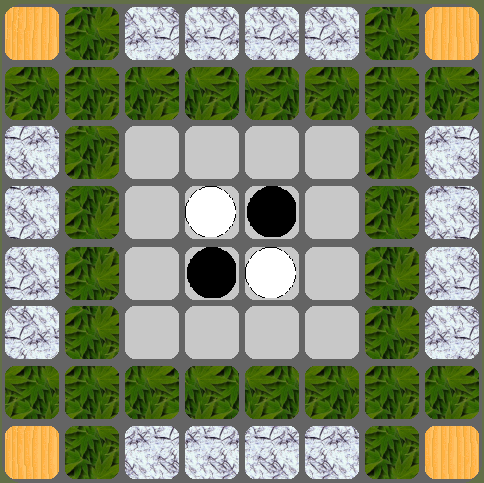
\includegraphics[width=0.3\textwidth]{img/eval_0.png}
    \end{center}
    \textbf{Les coins sont en or, les bords en argent, et le centre est dangereux}
\end{frame}

\begin{frame}[t,fragile]{Méthode d'évaluation}
    \textbf{Première idée:}
    Une matrice de pondération
    \begin{lstlisting}[basicstyle=\scriptsize, escapeinside={(*}{*)}]
def evaluate_board(self, board) -> float:
    WEIGHTS = [
        [150, -50, 20, 10, 10, 20, -50, 150],
        [-50, -50, -2, -2, -2, -2, -50, -50],
        [20, -2, 1, 1, 1, 1, -2, 20],
        [10, -2, 1, 0, 0, 1, -2, 10],
        [10, -2, 1, 0, 0, 1, -2, 10],
        [20, -2, 1, 1, 1, 1, -2, 20],
        [-50, -50, -2, -2, -2, -2, -50, -50],
        [150, -50, 20, 10, 10, 20, -50, 150]
    ]
    
    score = 0
    for i in range(8):
        for j in range(8):
            if board.get_at(i, j) == board._current_player:
                score += WEIGHTS[i][j]
            elif board.get_at(i, j) == 1 - board._current_player:
                score -= WEIGHTS[i][j]
    return score
    \end{lstlisting}
\end{frame}

\begin{frame}[t]{Méthode d'évaluation}
    \textbf{Les limites de la matrice de pondération}
    \begin{center}
        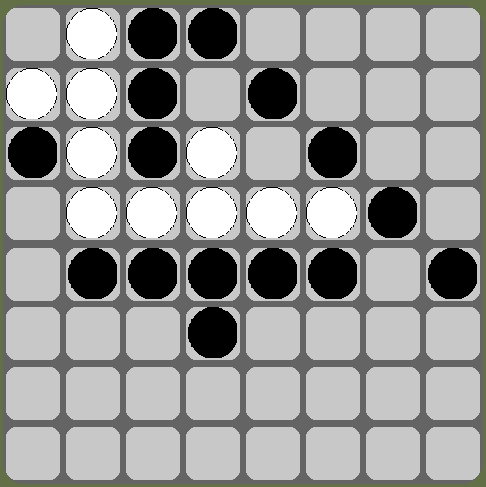
\includegraphics[width=0.2\textwidth]{img/matrix_0.png}
        \hspace{0.2\textwidth}
        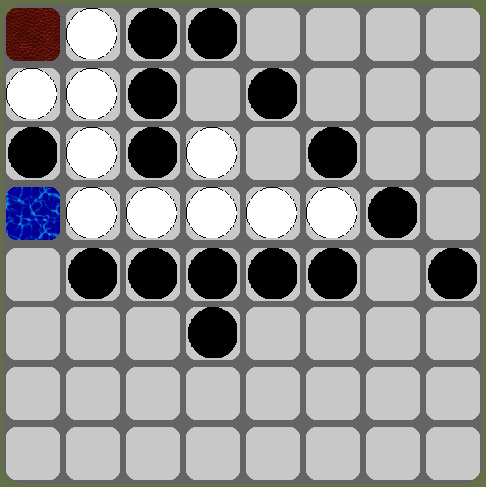
\includegraphics[width=0.2\textwidth]{img/matrix_1.png}
    \end{center}
    \begin{center}
        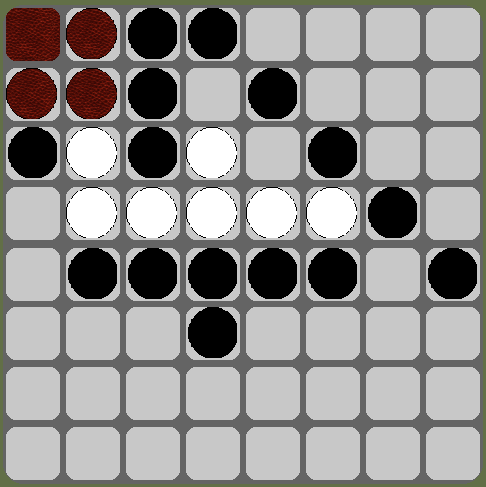
\includegraphics[width=0.2\textwidth]{img/matrix_2.png}
        \hspace{0.2\textwidth}
        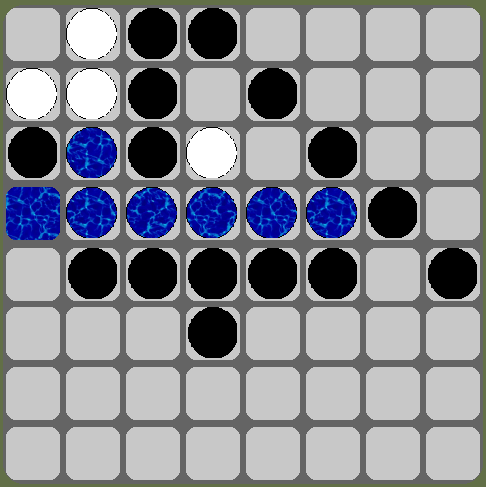
\includegraphics[width=0.2\textwidth]{img/matrix_3.png}
    \end{center}
    \textbf{Points:}
    \begin{itemize}
        \item Case rouge jouée: +150 -50 -50 -50 = 0
        \item Case bleue jouée: +10 -2 -2 +1 +1 = 8
    \end{itemize}
\end{frame}

\begin{frame}[t]{Méthode d'évaluation}
    \textbf{La version finale de la méthode d'évaluation}
    \begin{itemize}
        \item Différence de pions (P)
        \item Mobilité (M)
        \item Contrôle des coins (C)
        \item Stabilité (S)
        \item Danger des cases adjacentes aux coins (D)
    \end{itemize}
    \vspace{1.5em}
    \[
        P = 100 \times \frac{p_{IA} - p_{adverse}}{p_{IA} + p_{adverse}}
    \]
    \vspace{0.8em}
    \[
        M = 100 \times \frac{m_{IA} - m_{adverse}}{m_{IA} + m_{adverse}}
    \]
    \vspace{0.6em}
    \[
        C = 25 \times {(c_{IA} - c_{adverse})}
    \]
\end{frame}

\begin{frame}[t]{Méthode d'évaluation}
    \textbf{Danger des cases adjacentes aux coins}
    \hspace{0.2\textwidth}
    \begin{center}
        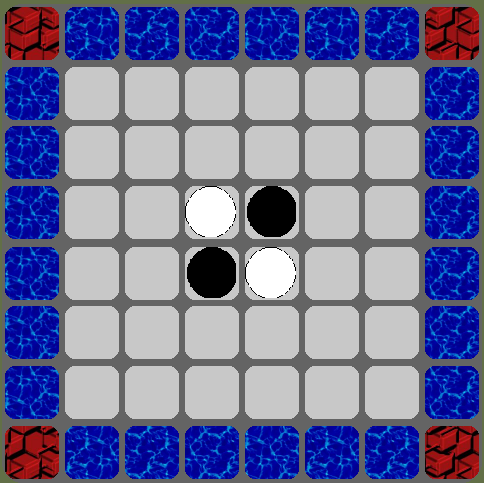
\includegraphics[width=0.35\textwidth]{img/stabilite.png}
    \end{center}
    \[
        s_{IA} = s_{IAc} \times 2 + s_{IAb} \times 1
    \]
    \[
        s_{adverse} = s_{adversec} \times 2 + s_{adverseb} \times 1
    \]
    \[
        S = 100 \times \frac{s_{IA} - s_{adverse}}{s_{IA} + s_{adverse}}
    \]
\end{frame}

\begin{frame}[t]{Méthode d'évaluation}
    \textbf{Danger des cases adjacentes aux coins}
    \hspace{0.2\textwidth}
    \begin{center}
        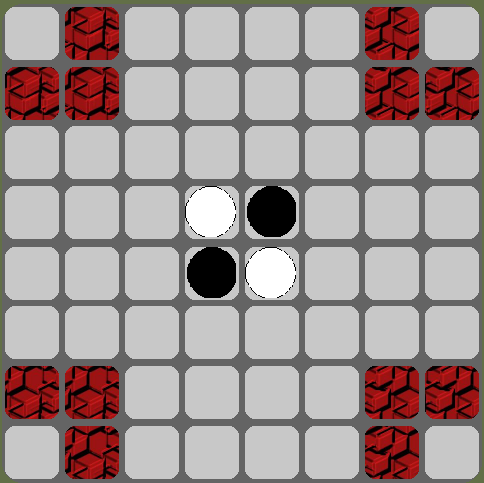
\includegraphics[width=0.37\textwidth]{img/danger_adj.png}
    \end{center}
    \hspace{0.5\textwidth}
    \[
        D = 12.5 \times \frac{d_{adverse} - d_{IA}}{1.5}
    \]
\end{frame}

\begin{frame}[t]{Méthode d'évaluation}
    \begin{block}{Formule globale}
        \[
        \text{Score} = w_P \cdot P + w_S \cdot S + w_M \cdot M + w_C \cdot C + w_D \cdot D
        \]
    \end{block}
    
    \begin{columns}[onlytextwidth,T]
        \column{0.33\textwidth}
        \begin{block}{\footnotesize Début de partie\\ (moins de 20 pions)}
            \scriptsize
            \setlength{\leftmargini}{0pt}
            \begin{itemize}
                \item[] Mobilité (150)
                \item[] Contrôle des coins (250) 
                \item[] Différence de pions (2)
                \item[] Stabilité (30)
                \item[] Adjacent coins (-100)
            \end{itemize}
        \end{block}
        
        \column{0.33\textwidth}
        \begin{block}{\footnotesize Milieu de partie\\ (20-50 pions)}
            \scriptsize
            \setlength{\leftmargini}{0pt}
            \begin{itemize}
                \item[] Mobilité (70)
                \item[] Contrôle des coins (600) 
                \item[] Différence de pions (25)
                \item[] Stabilité (120)
                \item[] Adjacent coins (-50)
            \end{itemize}
        \end{block}
        
        \column{0.33\textwidth}
        \begin{block}{\footnotesize Fin de partie\\ (plus de 50 pions)}
            \scriptsize
            \setlength{\leftmargini}{0pt}
            \begin{itemize}
                \item[] Mobilité (5)
                \item[] Contrôle des coins (2000) 
                \item[] Différence de pions (300)
                \item[] Stabilité (200)
                \item[] Adjacent coins (-5)
            \end{itemize}
        \end{block}
    \end{columns}
    
    \vspace{0.1cm}
    \centering
    \tiny
    * Les valeurs montrent l'évolution stratégique selon la phase de jeu
\end{frame}

\begin{frame}[t,fragile]{MinMax et l'élagage Alpha-Beta}
    \hspace{0.15\textwidth}
    \begin{lstlisting}[basicstyle=\tiny, mathescape=false]
def minimax(self, board, depth: int, alpha: float, beta: float, maximizing_player: bool):
    valid_moves = board.get_valid_moves()
    if depth == 0 or not valid_moves:
        return self.evaluate_board2(board)

    if maximizing_player:
        value = float('-inf')
        for move in valid_moves:
            board_copy = deepcopy(board)
            board_copy.make_move(*move)
            value = max(value, self.minimax(board_copy, depth - 1, alpha, beta, False))
            alpha = max(alpha, value)
            if beta <= alpha:
                break  
        return value
    else:
        value = float('inf')
        for move in valid_moves:
            board_copy = deepcopy(board)
            board_copy.make_move(*move)
            value = min(value, self.minimax(board_copy, depth - 1, alpha, beta, True))
            beta = min(beta, value)
            if beta <= alpha:
                break 
        return value
    \end{lstlisting}
\end{frame}

\begin{frame}
    \frametitle{MinMax et l'élagage Alpha-Beta}
    \centering
    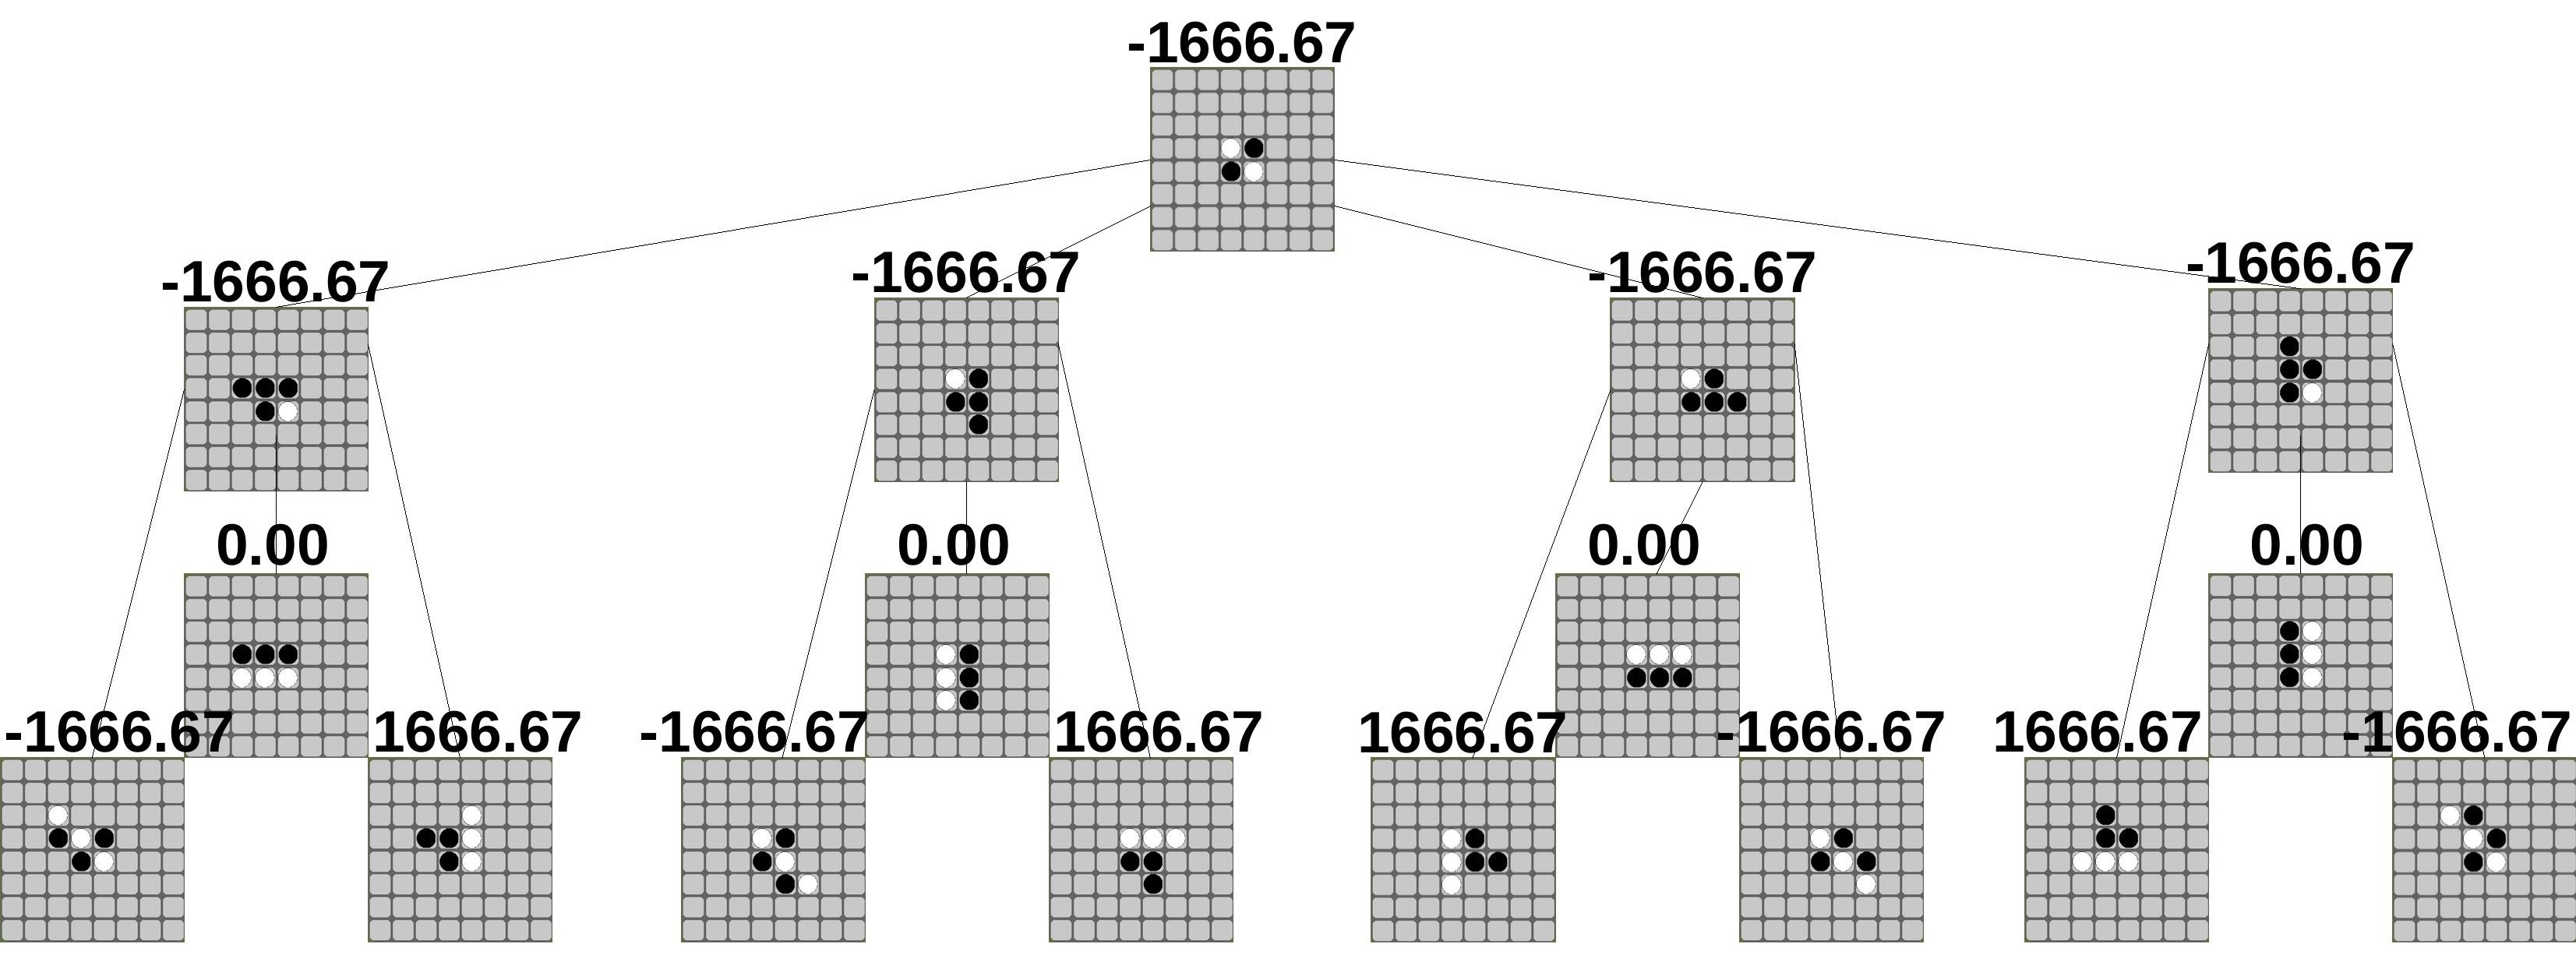
\includegraphics[width=1\textwidth]{img/minmax_eval.jpg}
    \[
    \mathrm{Score} = w_P \cdot P + w_S \cdot S + w_M \cdot M + w_C \cdot C + w_D \cdot D
    \]
    \begin{equation*}
    1666.67 = 2 \times 0 + 30 \times 0 + 150 \times \left(100 \times \frac{5-4}{5+4}\right) + 250 \times 0 + (-100) \times 0
    \end{equation*}
\end{frame}

\begin{frame}
    \frametitle{MinMax et l'élagage Alpha-Beta}
    \centering
    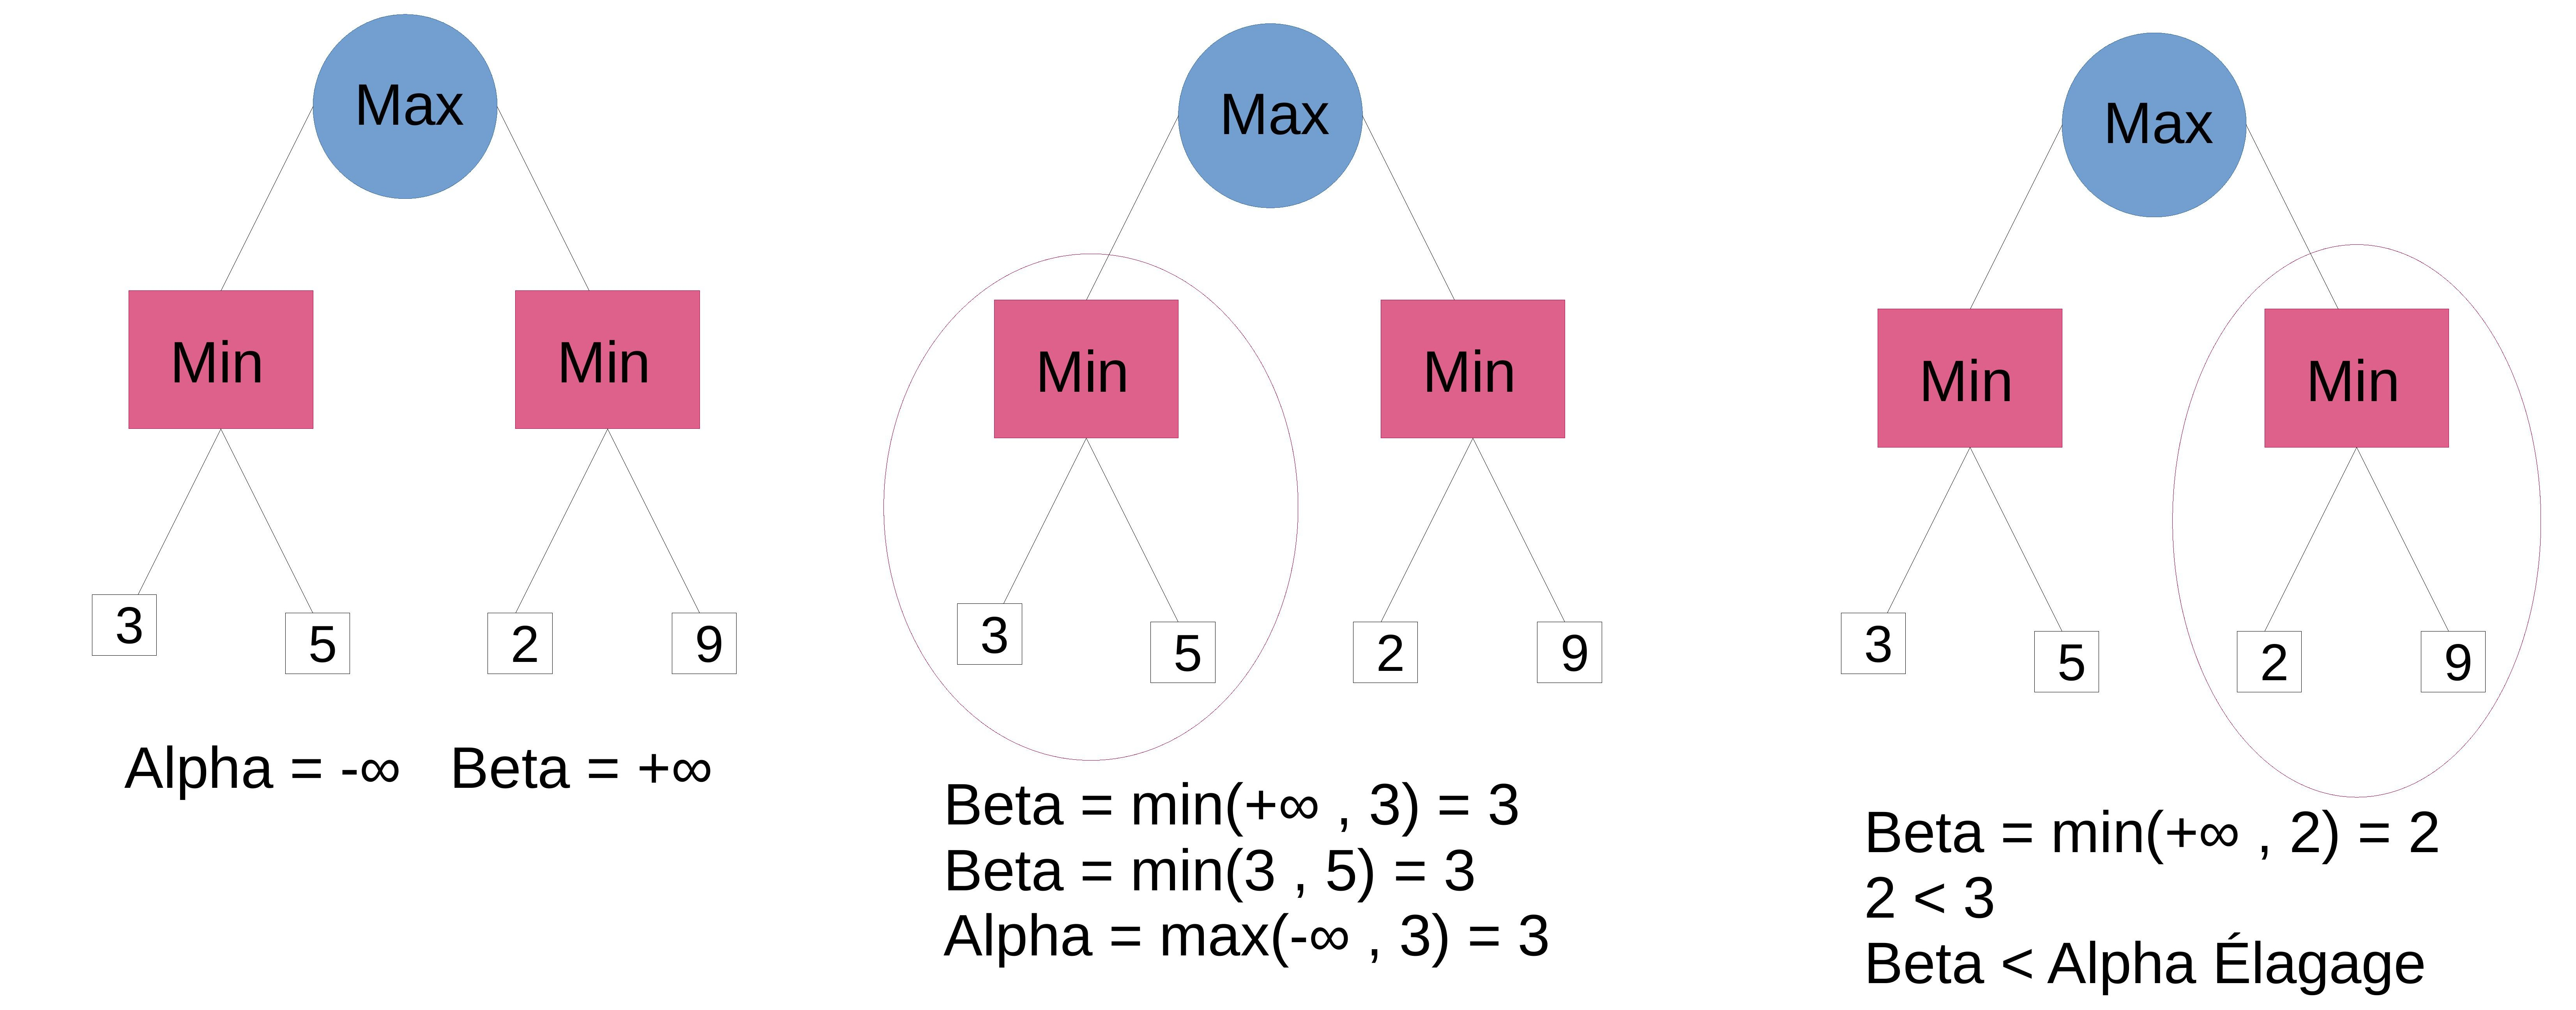
\includegraphics[width=1\textwidth]{img/alphabeta.jpg}
\end{frame}